\section{Low Energy Excess Overview and Motivation}
\subsection{Introduction}
The purpose of this chapter is to describe the MicroBooNE analysis centered around measuring the observed low energy excess as seen by its predicessor experiment, MiniBooNE. This chapter begins with a historical motivation for this analysis by describing the LSND experiment which first observed an excess of $\overline{\nu_e}$ in a $\overline{\nu_\mu}$. Then, a detailed description of the MiniBooNE experiment (detector and analysis) is provided, which observed an unexplained excess of electron-like events in the neutrino energy region between 200 to 475 MeV.\\

With historical context in perspective, this chapter then discusses an analysis conducted which determines the sensitivity of the previously described MicroBooNE detector to measure the same signal as MiniBooNE, assuming that signal originated from an excess of beam-induced $\nu_e$ interactions. This discussion covers the signal modeling which comes from MiniBooNE published data releases, the event selection and background mitigation techniques in MicroBooNE, and ultimately the expected sensitivity to measure such a signal.

\subsection{LSND Observation}
%Brief discussion of the LSND experiment and how they saw an excess of antinue in the antinumu beam with L/E that didn't fit in with any measured mixing angles and delta m2 in 3 neutrino model.

In 2001, the Liquid Scintillator Neutrino Detector (LSND) collaboration published an observation of excess events consistent with $\overline{\nu_e}$ interactions above the expected background in an $\overline{\nu_\mu}$ beam at the Los Alamos Neutron Science Center \cite{LSNDPaper}. The $\frac{L}{E}$ ($\approx$ $\frac{30 m}{40 MeV}$) for this excess disagreed with previous measurements of neutrino mixing angles and $\Delta m^2$ values in the three neutrino model. The LSND excess corresponded to a $\Delta m^2$ of approximately 1 $eV^2$, significantly higher than previously measured values of $\Delta m_{12}^2$ and $\Delta m_{23}^2$. One explanation for this drastically different $\Delta m^2$ value is the existance of potential additional ``sterile'' neutrino states, which must not interact weakly given the Z- boson decay width constrains the number of weakly interacting neutrino states to three.\\
To test the LSND result, the MiniBooNE experiment was designed. It would similarly measure $\nu_e$ interactions in a primarily $\nu_\mu$ beam, with a similar $\frac{L}{E}$ ($\approx$ $\frac{500m}{700 MeV}$).



\subsection{The MiniBooNE Experiment}

\subsubsection{The MiniBooNE Detector and Monte Carlo Simulation}

%Description of the detector, a schematic figure, description of cherenkov rings, the location of the detector in the BNB. Discussion of how they use NUANCE, mention they use identical beam simulation and reweighting (reweighting should be covered in the beam chapter).


The MiniBooNE detector \cite{MBDetectorPaper} consists of a spherical tank located 541 meters downstream of the BNB neutrino production target, with diameter of 12.2 meters filled with 818 tons of mineral oil underneath at least 3 meters of earth overburden as shown in Figure \ref{MB_detector_fig}. As seen in the figure, there exists an opaque barrier separating a veto region and a signal region. The walls of the signal region are painted black to reduce re-scattering of light and are instrumented with 1280 8-inch photomultiplier tubes (PMTs), most of which were reused from the LSND experiment. In the signal region, the photocathode coverage is 11.8\%. This region is intended to identify beam neutrino interactions happening within it; the PMTs face radially inwards. The veto region is 35 cm thick and is instrumented with 240 PMTs which face tangent to the detector radius and its purpose is to reject backgrounds coming from outside of the detector (cosmics, which have a rate at the detector location of about 10 kHz). The inner surface of the veto region is coated in a reflective paint. The efficiency for rejecting cosmic ray muons with the outer veto region was measured to be 99.99\%.\\

\begin{figure}[ht!]
\centering
	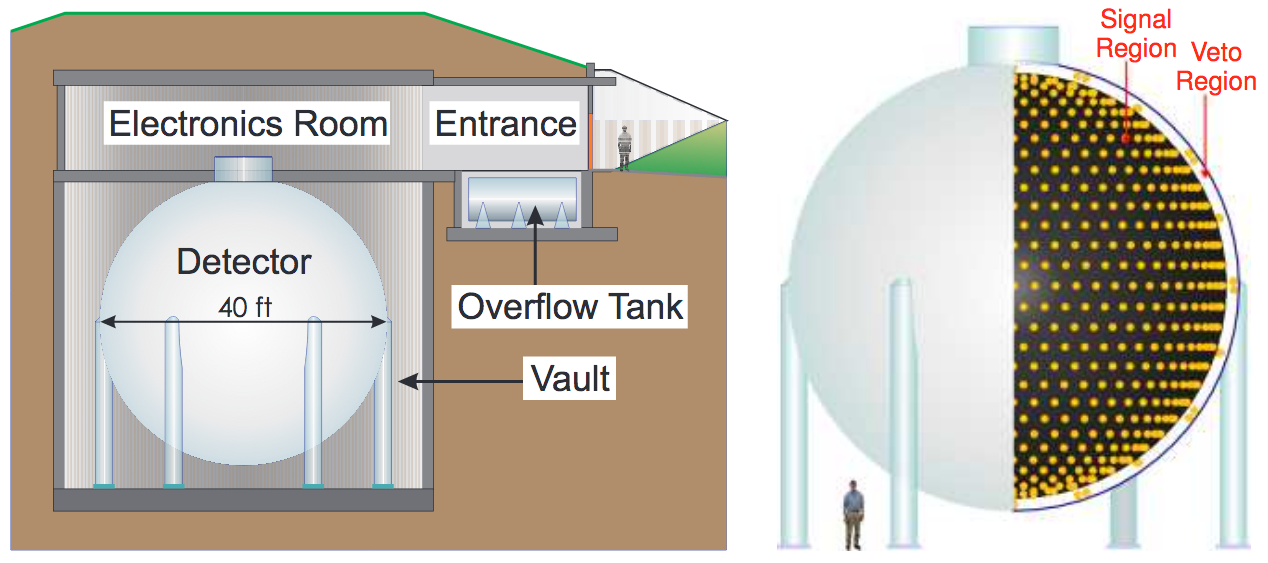
\includegraphics[width=0.9\textwidth]{Figures/MB_detectorpaper_fig.png} \\
\caption{\textit{The MiniBooNE detector enclosure (left) and a cut-away drawing (right) of the detector showing the distribution of PMT's in the signal and veto regions.}}\label{MB_detector_fig}
\end{figure}

The detection method of the MiniBooNE experiment is based primarily on Cherenkov light. The mineral oil within the signal region acts as the neutrino target material. The majority of final state particles exiting neutrino interactions at neutrino energies from the BNB are produced above Cherenkov threshold. These particles produce Cherenkov light which is detected by the PMTs lining the signal region of the detector. Reconstructing the pattern this light projects onto the walls of the signal region allows for some particle identification abilities.\\

Thie mineral oil used in MiniBooNE is Marcol 7 Light Mineral Oil ($CH_2$). While the oil has lower density than water (a common material choice for Cherenkov detectors) and therefore smaller probability of a neutrino interacting within the detector, the other benefits outweigh this downside. The oil has good light transmission throughout the wavelength range of 320 nm to 600 nm, relatively large refractive index (1.47, greater than water at 1.33), and its long extinction length of greater than 20 m for 420 nm light. This extinction length allows for loss of no more than 25\% of light generated by a neutrino interaction at the center of the detector. Additionally, the Cherenkov threshold is lower than that of water for the final state particles of interest (electrons, pions, muons, protons), allowing for the measurement of lower energy particles.\\

The PMTs have a wavelength dependent efficiency with a peak at 390 nm, with half that efficiency at 315 and 490 nm. They are operated at +2000 V which results in a gain of approximately $1.6 \times 10^7$. They have an intrinsic time resolution on the order of 1 ns, which is the dominant contribution to the final time resolution in the final PMT data after readout through data acquisition (DAQ) electronics. The DAQ reads out a pmt when the charge signal corresponds to more than 0.1 photoelectrons (PE). The deadtime between successive PMT readouts is on the order of 250 ns after the first readout began. PMT charge and timing information is stored in intervals of 200 $\mu s$ following any trigger signal. The trigger signal of interest for this analysis is the beam trigger which is induced by the BNB accelerator clock such that the DAQ begins readout 5 $\mu s$ before each beam spill.\\

The detector is calibrated in situ primarily from cosmic ray muons. Within the detector are six optically sealed scintillator cubes. Incominb muons are tagged with a muon hodoscope above the detector with angular resolution better than 2 degrees. Those muons that stop within one of the scintillation cubes have well defined energy (in the 100-800 MeV range), as the stopping power of muons in mineral oil is well known, and therefore provide an energy calibration source. Additionally, the outgoing electrons from stopping muon decay (Michel electrons) have a well known endpoint of around 50 MeV and therefore serve as an electron energy calibration source at that energy. Through-going muons are also used as an energy calibration source at higher energies (above 1 GeV). Additional calibration sources include a laser system built into the detector, and reconstructed $\pi^0$ masses (with peak energy at 135 MeV).

\subsubsection{MiniBooNE Event Selection and Observed Excess}
% Brief description of their event selection cuts, mention that the energy definition they use is CCQE and they're looking specifically for CCQE topologies, description of what CCQE means. Figure of their results indicating the excess in neutrino mode. 

Different final state particles exiting a neutrino interaction in the MiniBooNE signal volume will create different patterns of Cherenkov light read out by the PMTs. Figure \ref{georgia_cherenkov_cartoon_fig} \cite{GeorgiaThesis} shows how these patterns differ for different common kinds of final state particles (muons, electrons/photons, and neutral pion decays). A muon track produces a crisp, filled-in ring of Cherenkov light, while an electron or photon produces a more fuzzy, hollow ring. A neutral pion decay will result in two photons. By reconstructing these patterns in the PMT data read out from a triggered event in MiniBooNE, the flavor and energy of the interacting neutrino can be determined. With this kind of detection technique it is important to note that a single photon signal is indistinguishable from that of a single electron signal, an important ingredient to the ultimate ambiguity of the observed low energy excess in MiniBooNE.\\

\begin{figure}[ht!]
\centering
	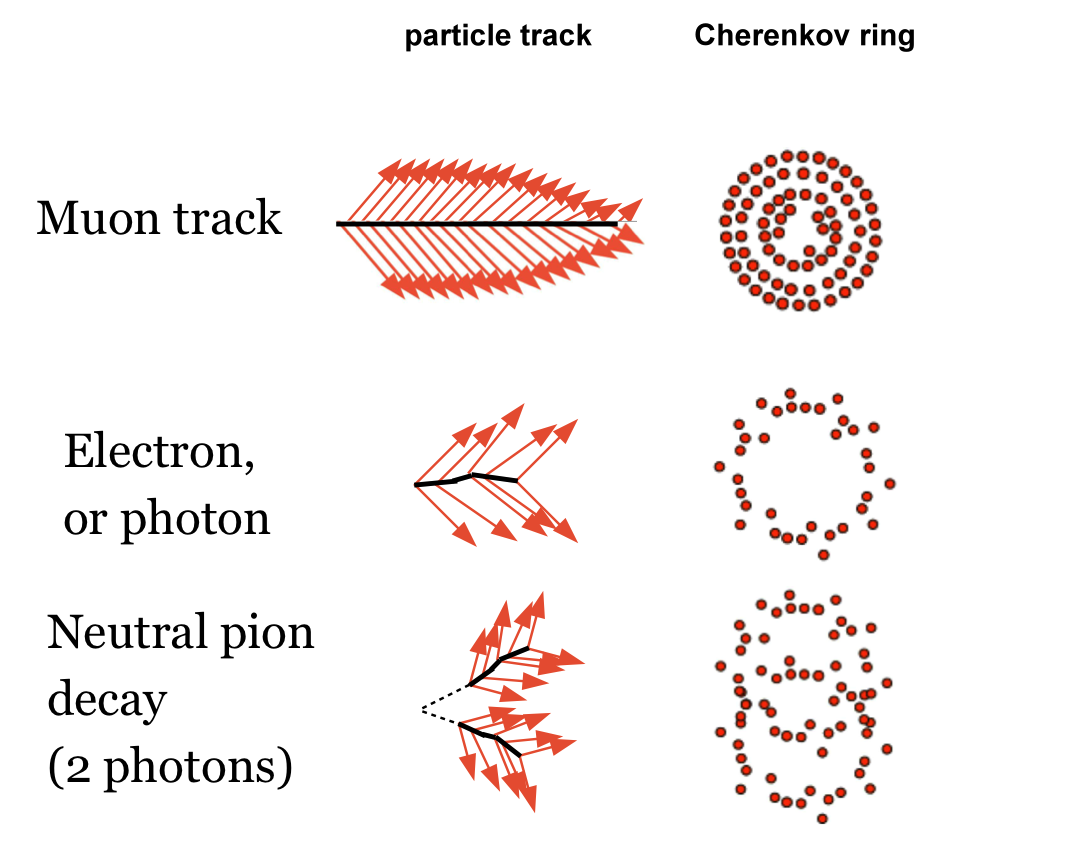
\includegraphics[width=0.9\textwidth]{Figures/georgia_cherenkov_cartoon.png} \\
\caption{\textit{A schematic of the pattern Cherenkov light from different particles would make projected onto the inner walls of the MiniBooNE detector. Top is a muon track (a filled-in ring), middle is an electron (a fuzzy ring), bottom is a photon that pair-produces and creates two fuzzy rings.}}\label{georgia_cherenkov_cartoon_fig}
\end{figure}

The topology of interest in the MiniBooNE oscillation search is that of charged-current quasi-elastic (CCQE) interactions, shown in Figure \ref{georgia_ccqe_feynman_fig}. This interaction channel is the dominant one in the neutrino energy range of the BNB, around 1 GeV $E_\nu$. In a $\nu_l$ CCQE interaction (where $l$ is the neutrino flavor), a lepton of flavor $l$ is produced, along with a proton. The single outgoing lepton is the characteristic event signature for which MiniBooNE searches.\\


\begin{figure}[ht!]
\centering
	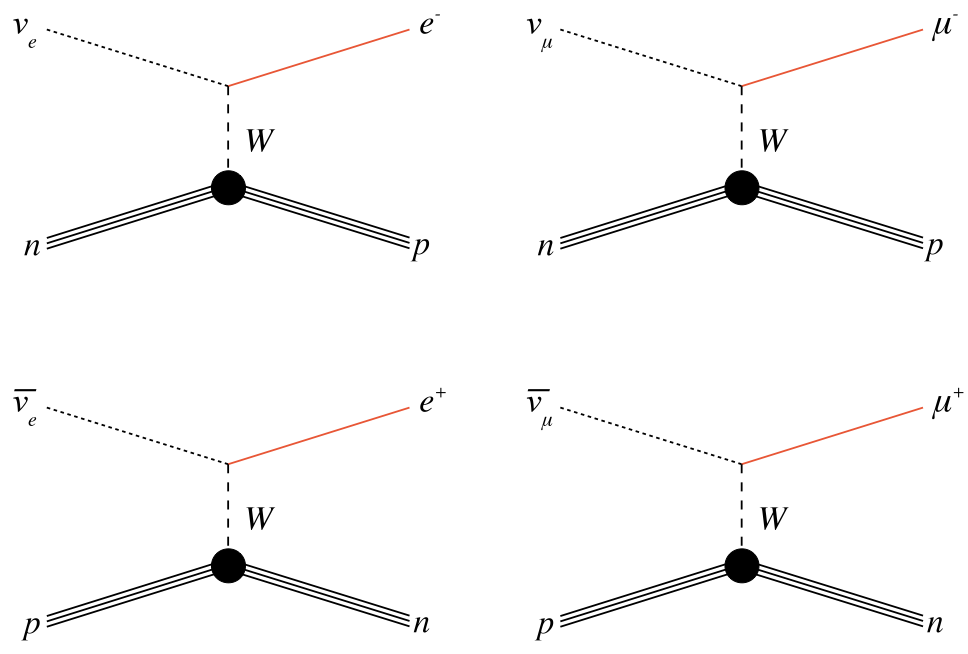
\includegraphics[width=0.9\textwidth]{Figures/georgia_ccqe_feynman.png} \\
\caption{\textit{Feynman diagrams of the charged-current quasi-elastic (CCQE) interaction channel for $\nu_e$, $\nu_\mu$, $\overline{\nu_\mu}$, and $\overline{\nu_e}$ (clockwise from the top left). $\nu_e$ CCQE is the signal channel for the MiniBooNE oscillation analysis.}}\label{georgia_ccqe_feynman_fig}
\end{figure}


In order to select $\nu_e^{CCQE}$ events, cuts are placed to mitigate backgrounds. The most powerful rejection comes from requiring the events occur within the beam timing window. Two additional cuts are used that require there be more activity within the signal volume than the outer veto volume, a signature characteristic of beam related neutrino events. These pre-cuts achieve more than a 99.99\% rejection of beam unrelated backgrounds.\\

In order to reconstruct events, MiniBooNE uses a maximum likelihood fitting algorithm leveraging properties of charged particle tracks inferred from measured charges and times on the PMTs. The likelihoods to different event hypothesis are used to classify each event as a signal $\nu_e$ CCQE event, or as a background process like $\nu_\mu$ CCQE and NC $\pi^0$ production. Note that MiniBooNE cannot differentiate between a $\mu^+$ and a $\mu^-$, or $e^+$ and $e^-$ so discrimination between neutrino and antineutrino on an event-by-event basis is impossible.\\

Assuming CCQE kinematics, the incident neutrino energy is reconstructed with knowledge of the outgoing lepton energy ($E_l$) and scattering angle ($\theta_l$). In MiniBooNE specifically, the struck nucleon is assumed to be at rest, so the incident neutrino energy $E_\nu^{CCQE}$ is given by:

\begin{equation}\label{MB_CCQE_formula}
E_\nu^{CCQE} = \frac{2m_nE_l+m_p^2-m_n^2-m_l^2}{2(m_n-E_l+\cos\theta_l\sqrt{E_l^2-m_l^2})}
\end{equation}

where $m_n$, $m_p$, $m_l$ are the masses of the neutron, proton, and lepton respectively, and $\theta_l$ is the scattering angle of the outgoing lepton with respect to the (known) beam neutrino direction.\\

With the described reconstruction methods and energy definition, the MiniBooNE published results \cite{MBLEEPaper} for the $\nu_e$ appearance search in neutrino mode running are shown in Figure \ref{MB_published_stackedhisto_fig}. There is clearly a statistically significant excess of events below $E_\nu^{CCQE}$ of 475 MeV. Note that besides the irriducible intrinsic $\nu_e$ backgrounds, the dominant background in the excess region is $\pi^0$ MID (red). In a $\pi^0$ MID event event, a $\pi^0$ is created in the neutrino interaction and its subsequent immediate decay into two photons mimics a the $\nu_e$ CCQE signature (either one photon escapes, or rings overlap). Another important background is $\Delta\rightarrow N\gamma$ (brown). Recall that both of these backgrounds arise from MiniBooNE's inability to distinguish electrons from photons.\\


\begin{figure}[ht!]
\centering
	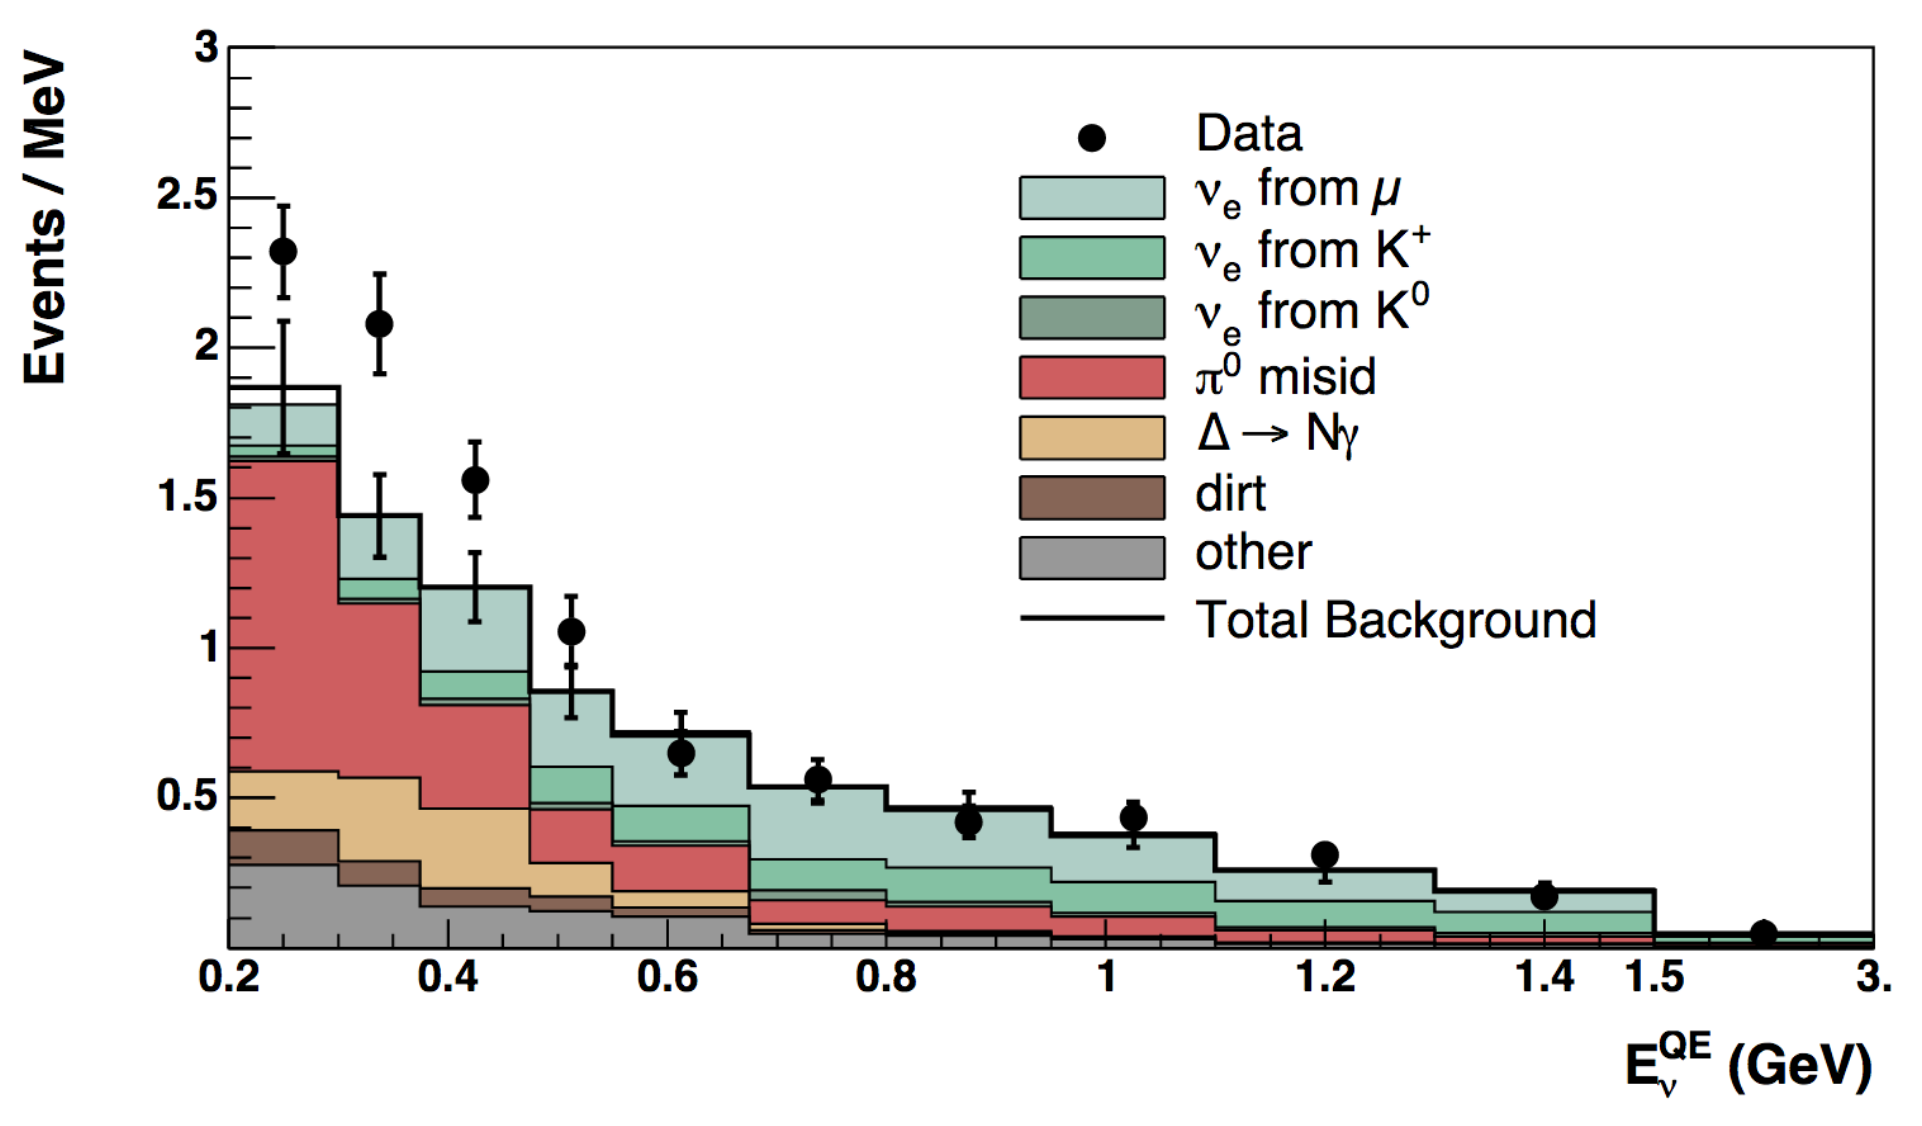
\includegraphics[width=0.9\textwidth]{Figures/MB_published_stackedhisto.png} \\
\caption{\textit{The $E_\nu^{QE}$ distribution for MiniBooNE data (points with statistical errors) and and backgrounds (histogram with systematic errors).}}\label{MB_published_stackedhisto_fig}
\end{figure}

\subsubsection{Proposed Low Energy Excess Sources}
% The LEE could either be electron like or photon like, MiniBooNE couldn't tell. Mention of theories like sterile neutrinos though no models seem to fit very well (3+1 or 3+2 with possible CP violation), single photon background misestimations or unexpected backgrounds, neutrino decay, lorentz violation etc etc. 
Shown in Figure \ref{MB_published_excess_fits_fig} is the MiniBooNE neutrino mode excess (data - expected background) with oscillation fits with parameters constrained to be in the LSND allowed region. The parameters in the LSND allowed region are ruled out at the 95\% confidence level if the data are fit with $E_\nu^{CCQE}$ > 475 MeV. \\

\begin{figure}[ht!]
\centering
	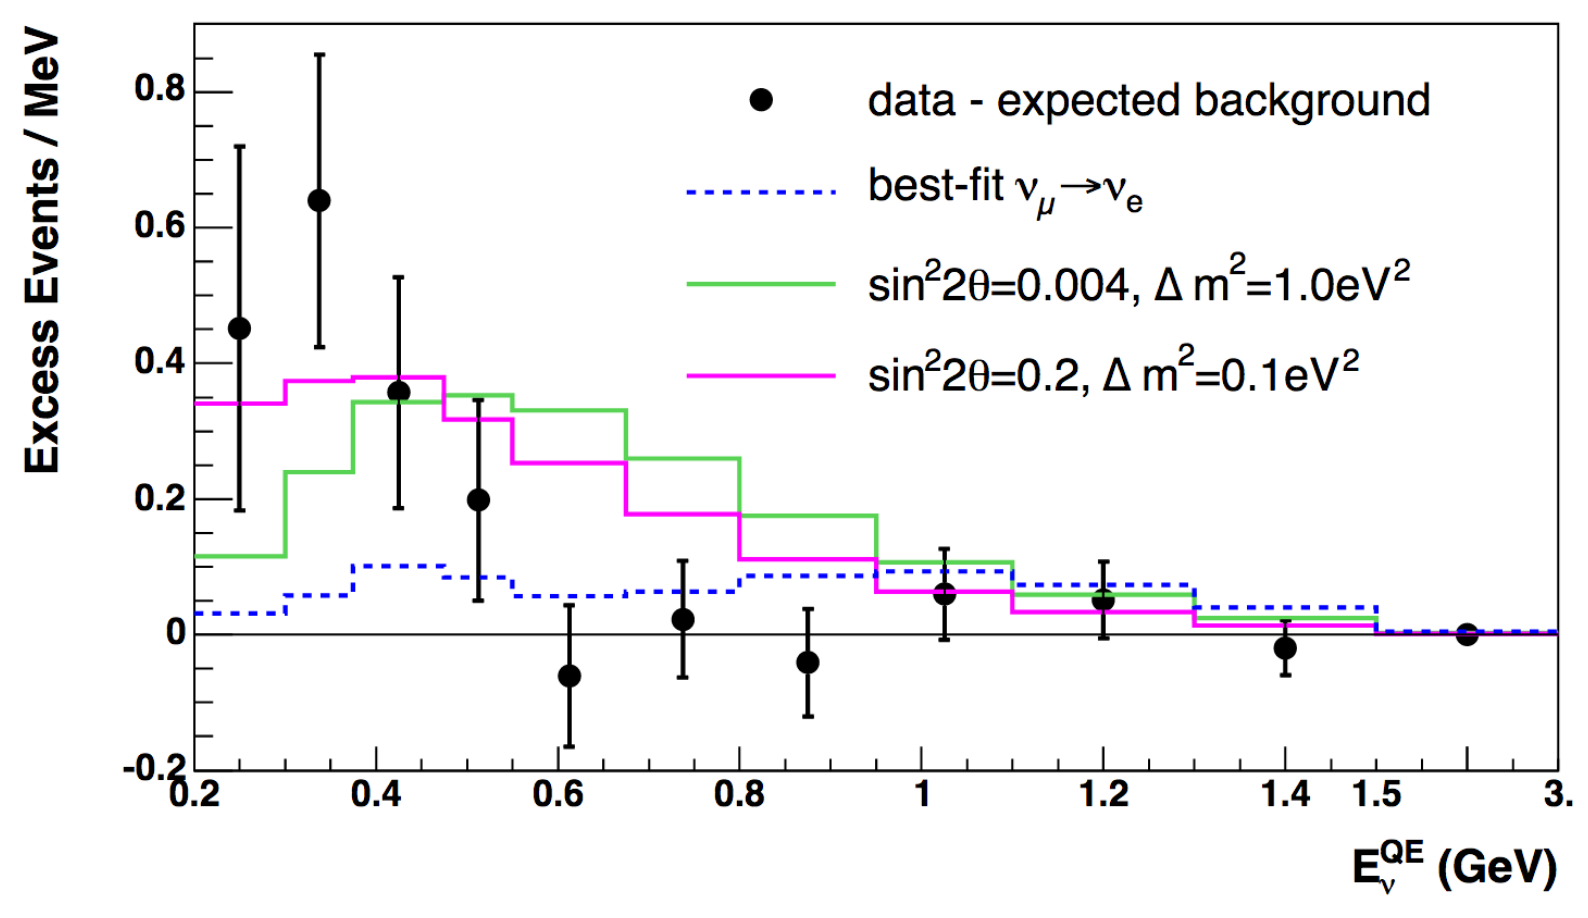
\includegraphics[width=0.9\textwidth]{Figures/MB_published_excess_fits.png} \\
\caption{\textit{The MiniBooNE event excess as a function of $E_\nu^{QE}$. Also shown are the expectations from the best oscillation fit and from neutrino oscillation parameters in the LSND allowed region. The error bars include both statistical and systematic errors.}}\label{MB_published_excess_fits_fig}
\end{figure}

Given MiniBooNE's inability to distinguish electrons from photons, the origin of this excess is either a mis-estimation of one of the backgrounds, or some sort of new physics. The former is unlikely the case because MiniBooNE makes many \textit{in situ} measurements that allow for the constraining of these backgrounds. The neutral current induced backgrounds (NC $\pi^0$, $\Delta\rightarrow N\gamma$, and dirt) are constrained by such measurements.\\

The NC $\pi^0$ rate in MiniBooNE is measured by selecting events with reconstructed mass near the $\pi^0$ mass and obtains a $>90$\% pure sample of NC $\pi^0$ interactions which is compared to simulation to obtain a correction function in order to bring the simulated distribution in agreement with data. This same correction function is applied to NC $\pi^0$ events that are backgrounds in the $\nu_e$ appearance analysis. This correction function increases the NC $\pi^0$ background by less than 13\% for $E_\nu^{CCQE}$ $<$ 400 MeV and decreases the background by as much as 20\% above this neutrino energy region. Including this correction factor, the uncertainty on the overall NC $\pi^0$ backgrounds is 7\%. Note that a correction factor of 2.0 would be required to explain the origin of the excess as originating from a misestimated NC $\pi^0$ background.(XXX citation here... got this from Georgia's thesis)\\

The excess is unlikely caused by a misestimation of the $\Delta\rightarrow N\gamma$ backgrounds because they are additionally constrained by the NC $\pi^0$ measurement through the relative rate of resonant production times a branching fraction of (0.56$\pm$0.04)\% (XXX citation here... got this from Georgia's thesis). With this measurement, the uncertainty on the $\Delta\rightarrow N\gamma$ backgrounds is 12\%. Note that a correction factor of 2.7 would be required to explain the origin of the excess as originating from a misestimated $\Delta \rightarrow N\gamma$ background.\\

The excess is unlikely caused by a misestimation of the dirt backgrounds because a direct measurement is made by selecting a separate event sample which are likely dirt events and comparing data to simulation. These events are reconstructed close to the detector boundaries with direction pointed generally inwards. In neutrino mode, a dirt background normalization correction factor was computed to be 0.7 $\pm$ 0.1 (with simulation over-predicting the dirt rate normalization). Given the power of the event selection cuts designed to mitigate dirt backgrounds, the relevance of this relatively large correction factor is minimal.\\

The charged current induced backgrounds (intrinsic $\nu_e$CCQE) are reduced with \textit{in situ} measurements of $\nu_\mu$CCQE interactions. A data to simulation comparison of measured $\nu_\mu$CCQE interactions allows for the retuning of underlying flux and cross section parameters in order to bring simulated distributions in agreement with data. These parameters are the same as those used to predict the $\nu_e$CCQE rate and shape. In addition, a measurement of the highest energy $\nu_\mu$CCQE interactions allows for the further constraint of $\nu_e$CCQE from kaon decay backgrounds, which is discussed in more detail in a later section of this thesis.\\

Given the likelihood that the excess is not caused by misidentified backgrounds, several new-physics interpretations have been proposed in attempt to explain the excess, including sterile neutrino oscillations (with one, two, or more sterile neutrinos), and new interactions both within and outside of the standard model (CPT violation, quantum decoherence, sterile neutrino decay, etc). A summary of these interpretations can be found in \cite{MBLEESourcesOverview}. A commonality between all interpretations is that their interactions pass the MiniBooNE event selection cuts; that is, they have one electron or one photon exiting the interaction vertex.

\subsection{MicroBooNE In The Context of the Low Energy Excess}
% Discussion of how as a LArTPC MicroBooNE has electron/photon separation. Showing the scaled signal plot from the TDR. Mention that this scaled signal is oversimplified so that's why this thesis describes a more rigorous sensitivity study with simulation in MicroBooNE.

%http://microboone-docdb.fnal.gov:8080/cgi-bin/RetrieveFile?docid=3528&filename=low-E-excess-note.pdf&version=2
Given the proposed explanations for the origin of the measured MiniBooNE low energy excess in neutrino mode all predict either a single electron or single photon produced at the neutrino interaction vertex, and that MiniBooNE cannot discriminate between single electrons or photons, the MicroBooNE experiment was proposed. This detector (described in detail in Section \ref{XXXMICROBOONEDETECTORSECTIONXXX}) is a liquid argon time projection chamber, a relatively new detector technology which allows for the discrimination between single electrons and photons based on the energy deposition at the start of their tracks (photons will pair produce and in general have twice the ionization as a single electron). MicroBooNE runs in the same beam line (BNB) in neutrino mode and is physically located very close to MiniBooNE. Therefore, MicroBooNE should be able to elucidate the MiniBooNE low energy excess ambiguity. \\

A preliminary attempt to scale the MiniBooNE backgrounds and excess to the MicroBooNE both under the assumption that the excess is due to an electron-like event (left) or under a photon-like event (right) \cite{UBTDR} is shown in Figure \ref{TDR_LEE_scaling_fig}. The resulting statistical significance after the nominal amount of data is taken in MicroBooNE ($6.6\times 10^20$ POT) is computed to be 5.7$\sigma$ under the single-electron excess hypothesis and 4.1$\sigma$ under the single-photon hypothesis. Note that this scaling is assuming the electron/photon misidentification rate in MicroBooNE is assumed to be 6\% (whereas it is 100\% for MiniBooNE). Also event selection efficiencies in MicroBooNE are assumed to be twice that of MiniBooNE because of the detector technology. This scaling procedure also ignores other potentially important differences between MicroBooNE and MiniBooNE including differences in detector geometry (important for $\pi^0$ misidentifications in which one photon escapes), flux differences (which are non-negligible despite the relative close physical proximity of the two detectors), event topology selection differences (MicroBooNE can see much more vertex activity than can MiniBooNE, especially when additional final state particles are below Cherenkov threshold), the differing cosmic rejection background efficiencies (MiniBooNE can reject cosmics much more efficiently than MicroBooNE), cross section differences between argon and $CH_2$ arising from differing proton to neutron ratios, among other things.\\

\begin{figure}[ht!]
\centering
	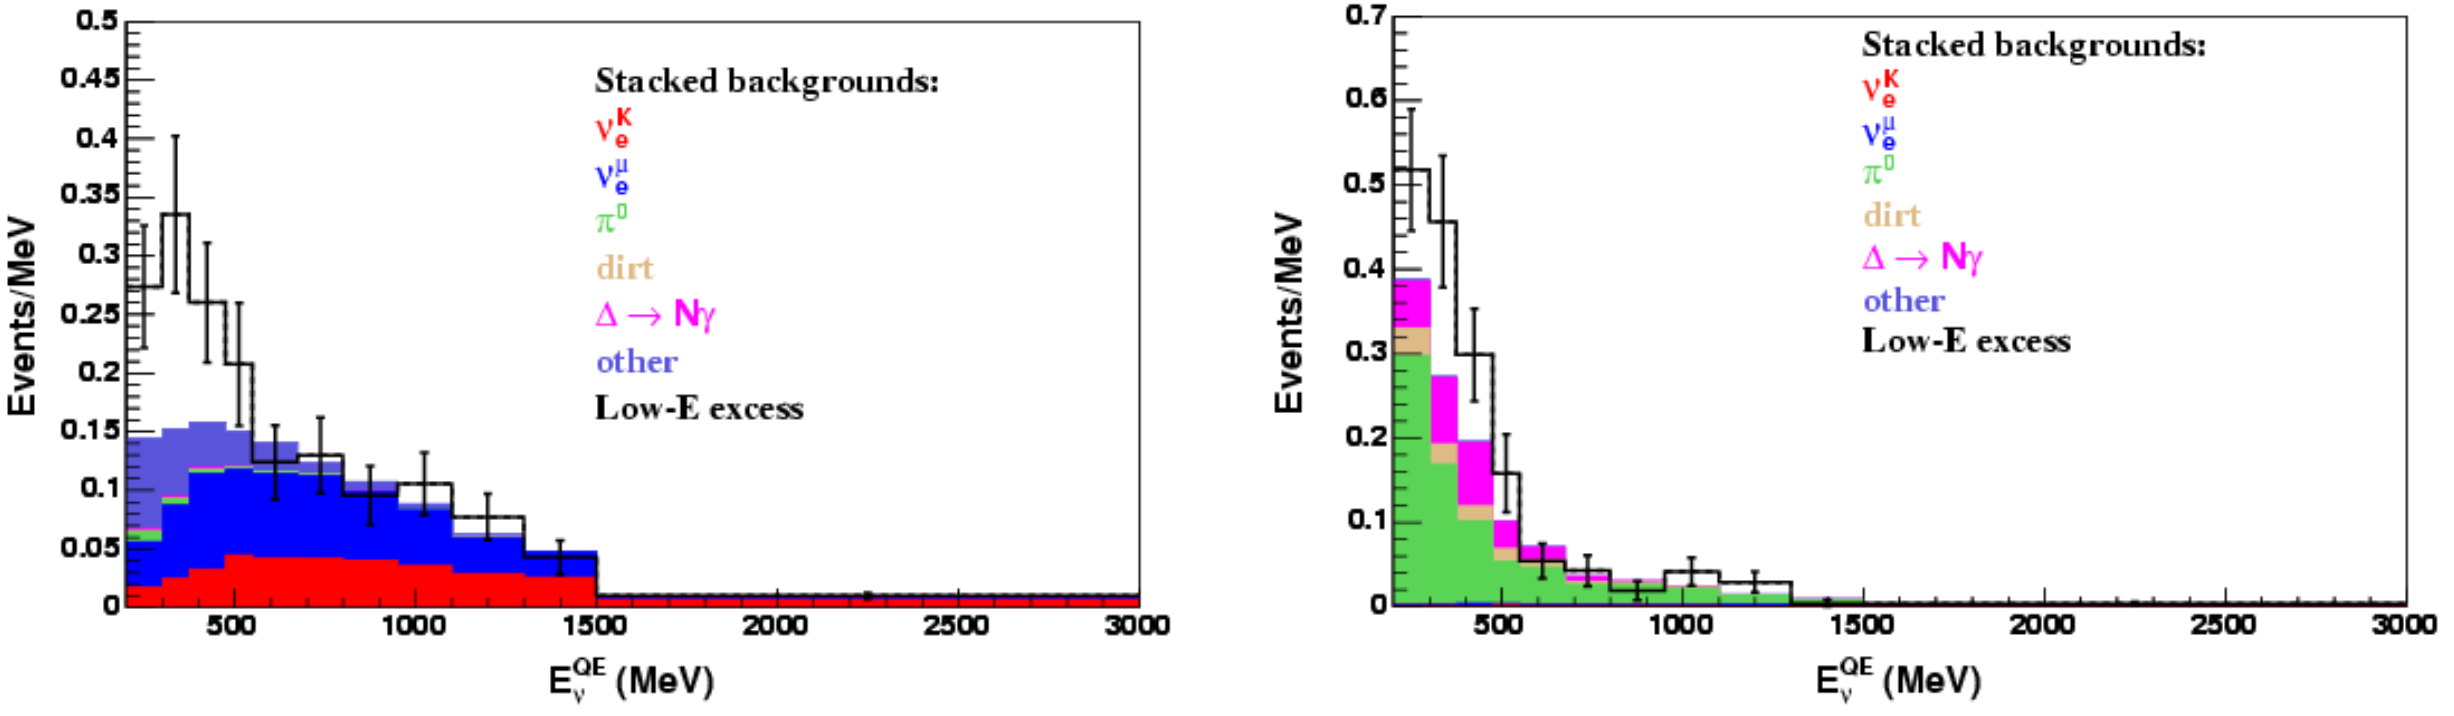
\includegraphics[width=0.9\textwidth]{Figures/TDR_LEE_scaling.png} \\
\caption{\textit{A preliminary attempt to scale the MiniBooNE backgrounds and excess to the MicroBooNE both under the assumption that the excess is due to an electron-like event (left) or under a photon-like event (right). Stacked histograms show the expected background. Error bars indicate statistical uncertainty. The number of signal events, scaled from MiniBooNE for neutrino flux and fiducial volume, is the same in both plots. Both plots assume $6.6 \times 10^20$ POT for the MicroBooNE 60 ton fiducial mass.}}\label{TDR_LEE_scaling_fig}
\end{figure}

While the aforementioned scaling of MiniBooNE backgrounds to MicroBooNE provides a reasonable estimate of the expected sensitivity to the MiniBooNE low energy excess, it is oversimplified for the reasons mentioned. The next sections in this thesis describe a more rigorous analysis with the ultimate goal of computing MicroBooNE's sensitivity to the MiniBooNE low energy excess assuming the single-electron hypothesis.














\section{Monte Carlo Simulation}

\subsection{Simulated Background Samples}
Mention that the input samples to this study are simulated BNB interactions inside of the entire cryostat, simulated cosmic samples, simulated intrinsic nue samples. Mention the stats are low because simulation is computationally intensive. Mention that GENIE is the generator. Mention the same flux reweighting is done as in MiniBooNE (and the same flux simulation is used as described in the beam chapter).

\subsection{Reconstruction}
Currently the automated reconstruction in MicroBooNE is not adequate to do any sort of sensitivity study (specifically shower reconstruction). Discussion that the input objects into this sensitivity are showers and tracks, description of what they are and how they differ. 
\subsubsection{``Perfect Reconstruction''}
Description of what {\sc MCTracks} and {\sc MCShowers} are, how they're made, etc. Make it clear that they are the input to the event reconstruction algorithms. Also make it clear that this entire sensitivity study is done only with these objects; no real automated reconstruction is covered (which is why no results on data are shown).



\section{Event Reconstruction}
This section describes how we take reconstructed objects (tracks and showers) and identify nue interactions. Mention that the analysis framework has many algorithms that each serve a specific purpose. Briefly mention the algorithms by name and what they're intended to do. Include the flowchart figure from the APS technote listing all the algorithms and the order in which they are executed. The following sections will describe in more detail the important ones. 

\subsection{Electron/Photon Separation Algorithm}
This is the algorithm (AlgoEMPart) that uses the reconstructed dE/dx and conversion distance to form a likelihood that a shower is electron like or photon like. It's one of the most important and should be described in detail. Include some figures showing performance of this algorithm.

\subsection{Nue Selection Algorithm}
This is the algorithm (AlgoSingleE) designed to look for the signal topology of CCInclusive... one electron plus anything else from the vertex. Mention the efficiency, etc.

\subsection{Energy Reconstruction}
Description of the energy definition. Mention that it is different than the CCQE energy definition MiniBooNE used. Include a figure of Ereco vs Etrue for the intrisic nue sample.



\section{Backgrounds}

\subsection{Background Topologies}
Description of the various background topologies (michel electrons from cosmics and numu, pi0s where one shower escapes, pi0s where one shower enters in dirt backgrounds, etc.)

\subsection{Background Normalization}
Mention the beam induced backgrounds are normalized to POT, the cosmic backgrounds come from the open cosmic sample and are normalized to beam gate open time (which is assuming perfect flash matching).

\subsection{Analysis Cuts and Results}
Description of the final cuts that are placed on the backgrounds (for example requiring the electron deposits more than 60 MeV of energy to mitigate michels, also requiring no pions in order to best mimic the MiniBooNE cuts). Showing the stacked backgrounds.



\section{MiniBooNE Low Energy Excess Signal Modeling In MicroBooNE}
Here is where I describe how I come up with my scaled signal shape and normalization. Simulated sample are intrinsic nues, since I'm assuming the excess is coming from beam nues. Shape comes from MiniBooNE published data (excess events evis distribution and uz distribution along with the CCQE formula). Normalization comes from size of MiniBooNE excess with respect to size of MiniBooNE intrinsic nue background in a specific region (excess should be larger than the intrinsic nue background in the low CCQE-energy region... this was Bill's recent suggestion). This section will probably be several pages long.

\subsection{Sensitivity Results}
Here I show the stacked background with the scaled signal on top, I describe how I compute a sensitivity (statistical errors only for now... I could do a back-of-the-envelope estimate of systematic errors which are dominated by flux). 
\subsubsection{Results with Realistic Shower Reconstruction Efficiency}
Here I mention that the ``perfect reconstruction'' efficiency is 100\% but that isn't quite realistic. I'll state we assumed 80\%, and ICARUS quoted something similar. I'll describe how we emulate the non-perfect efficiency and how it isn't as simple as multiplying everything by 0.8 (for example we will get increased pi0 backgrounds when we fail to reconstruct just one of the showers).
\subsubsection{Next Steps}
Here I talk about how what's next is automated shower reconstruction being incorporated. Another important ingredient in the whole LEE analysis is constraining the nue backgrounds. The intrinsic nues which come from kaon decay can be constrained by studying numu interactions that come from kaon decay. This section will flow into the next chapter of the thesis: kaon production studies.

